% !TeX root = ../../../book.tex

\subsection{像:定义与示例}

回想一下函数的定义。我们要求每个输入都有唯一一个输出,这确保了函数在其定义域上的每个元素都有定义。那么值域呢?我们只要求所有的输出都属于值域,但从未提及值域的``覆盖程度''。函数的像的概念正是为了说明这一点。正如我们将从一些例子中看到的那样,即使我们知道值域,确切地确定函数的像也并不总是容易的。正因为如此,我们才先定义了\emph{函数}及其\emph{值域},然后才引入\emph{像}的概念。所以请不要误会,我们并不是在试图误导你。

\subsubsection*{定义}

\begin{definition}
    设 $A, B$ 为集合,$f:A \to B$ 为函数。设 $X \subseteq A$。

    \dotuline{$X$ 在函数 $f$ 下的像} 写做 $Im_f(X)$,定义为
    \[Im_f(X) = \{b \in B \mid \exists a \in X \centerdot f(a) = b\}\]
    也就是说,$X$ 在函数 $f$ 下的像是集合 $X$ 中所有``输入''产生的``输出''的集合。

    一个等价的写法是
    \[Im_f(X) = \{f(a) \mid a \in X\}\]
    (当函数明确且无歧义时,我们有时会将符号简写为 $Im(X)$,并将其称为``$X$ 的像'',而不是``$X$ 在函数 $f$ 下的像''。)

    当我们说 \dotuline{$f$ 的像}时,我们指的是整个定义域的像,即 $Im_f (A)$。
\end{definition}

请注意,这一定义适用于定义域的任意子集 $X \subseteq A$,因此我们可以讨论定义域的任意``部分''或整个定义域的像。接下来我们看到的一些例子,以及稍后的练习中,都会涉及 $A$ 的真子集 $X \subset A$ 和整个集合 $A$。

\subsubsection*{一个发现}

请注意,\emph{无论} $f,A, B$ 是什么,都有
\[Im_f(A) \subseteq B\]
这是\emph{根据定义}得出的,因为我们使用集合构建符,通过 $B$ 的元素来定义像。在下一节中,我们将探讨当 $Im_f(A) = B$ 时会发生什么。

现在,让我们练习识别某些函数的像。有时,我们会提供一个函数及其像,并要求验证是否正确;而在其他情况下,我们需要先利用某些技术来确定像是什么。

\subsubsection*{示例}

\begin{example}\label{ex:example7.3.2}
    定义函数 $g : A \to B$ 为 $A = \{a, b, c, d, e\}, B = \{1, 2, 3, 4, 5, 6\}$ 且
    \[g = \{(a, 2),(b, 3)(c, 3),(d, 1),(e, 6)\}\]
    定义 $X_1 = \{a, b, c\}, X_2 = \{a, c, e\}, X_3 = \{c, d, e\}$。

    你可能已经注意到,这个函数与我们在上一节示意图中定义的函数是一样的!我们再来看一遍那个图,这有助于我们识别下面列表中的像。

    \begin{center}
        {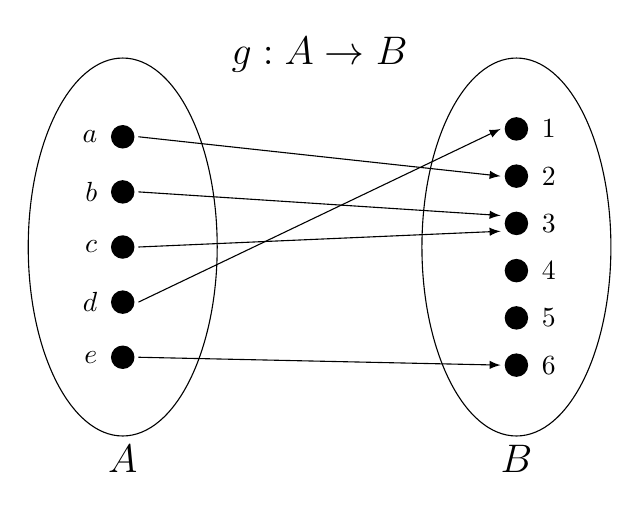
\begin{tikzpicture}[scale=1]
            \foreach \x in  {1,...,6}
            {
                \node at (5, -\x*0.6)[circle,fill,inner sep=3pt]{};
                \draw[shift={(5.2, -\x*0.6)}] node[right] {$\x$};
            }
            \draw (5,-2.1) ellipse (1.2 and 2.4);
    
            \foreach \x/\s in  {1/a,2/b,3/c,4/d,5/e}
            {
                \node at (0, -\x*0.7)[circle,fill,inner sep=3pt]{};
                \draw[shift={(-0.2, -\x*0.7)}] node[left] {$\s$};
            }
            \draw (0,-2.1) ellipse (1.2 and 2.4);
    
            \draw[-latex] (0.2,-0.7) -- (4.8,-1.2); 
            \draw[-latex] (0.2,-1.4) -- (4.8,-1.7); 
            \draw[-latex] (0.2,-2.1) -- (4.8,-1.9); 
            \draw[-latex] (0.2,-2.8) -- (4.8,-0.6); 
            \draw[-latex] (0.2,-3.5) -- (4.8,-3.6);
            
            \node[below] at (0, -4.5){\Large $A$};
            \node[below] at (5, -4.5){\Large $B$};
            \node[above] at (2.5, 0){\Large $g:A \to B$};
        \end{tikzpicture}}
    \end{center}

    \begin{enumerate}[label=(\arabic*)]
        \item $Im_g(\{a\}) = \{2\}$ \\
            因为 $g(a) = 2$。\\
            请注意这里\emph{大括号}的使用。我们找到永远都是\emph{集合}的像,因此写成 $\textcolor{red}{Im_g(a)}$ 是\emph{不正确的}。
        \item $Im_g(\{b, c\}) = \{3\}$ \\
            因为 $g(b) = g(c) = 3$。
        \item $Im_g(X_1) = \{2, 3\}$ \\
            因为 $g(b) = g(c) = 3, g(a) = 2$。
        \item $Im_g(X_2) = \{2, 3, 6\}$ \\
            因为 $g(a) = 2, g(c) = 3, g(e) = 6$。
        \item $Im_g(X_3) = \{1, 3, 6\}$ \\
            因为 $g(c) = 3, g(d) = 1, g(e) = 6$。
        \item $Im_g(A) = \{1, 2, 3, 6\}$ \\
            观察示意图中的集合 $B$,我们可以看到这些值是唯一被函数``命中''的。注意,虽然 $4,5 \in B$,但 $4,5 \notin Im_g(A)$,因此 $Im_g(A) \subset B$ ($Im_g(A)$ 是 $B$ 的\emph{真}子集)。
    \end{enumerate}
\end{example}

\begin{example}
    考虑水在液态时的温度范围(以摄氏度为单位)。具体来说,定义集合
    \[C = \{x \in \mathbb{R} \mid 0 < x < 100\}\]
    并且定义函数 $F : C \to \mathbb{R}$ 为
    \[\forall c \in C \centerdot F(c) = \frac{9}{5}c + 32\]
    $Im_F (C)$ 是什么?它具体代表什么?

    要解决此问题,我们需要
    \begin{enumerate}[label=(\alph*)]
        \item 通过定义一个集合来\emph{声明} $Im_F (C)$ 的含义;
        \item 证明我们定义的这个集合确实\emph{等于} $Im_F (C)$;也就是说他们在集合的意义上是相等的。 
    \end{enumerate}
    为此,我们将使用\emph{双重包含论证法}!

    \textbf{解}:定义 $S = \{y \in \mathbb{R} \mid 32 < y < 212\}$。(注意,这表示水在液态时的温度范围(以华氏度为单位)。) 我们声称 $S = Im_F (C)$。

    \begin{center}
        \begin{tikzpicture}
            \begin{axis}[
                ymin=0,
                ymax=220,
                xmin=0, 
                xmax=105,
                minor tick num=5,
                axis lines*=middle,
                xtick align=inside,
                ytick align=inside
                ]       
                \addplot[blue, line width=1pt, domain=0:100, samples=2] {x*1.8+32};
            \end{axis}
        \end{tikzpicture}
    \end{center}

    一般来说,很难给出如何提出这种主张的建议。通常,这需要对函数进行一些尝试和测试,可能还需要对函数的其他性质有一定洞察。在这个特定的例子中,我们注意到这个函数是递增的;也就是说,如果我们有两个输入值 $c_1 < c_2$,那么我们就知道 $F(c_1) < F(c_2)$。我们可以从函数的图像中(见上图)得出这一信息,或者认识到它是一个线性多项式。因此,为了确定函数的值域,我们只需要考虑最小输入值和最大输入值,并确定它们的输出。(同样,我们可以从图表中得出这一信息。)我们发现
    \[F(0) = 0 + 32 = 32 \qquad F(100) = \frac{900}{5} + 32 = 212\]
    由此,我们定义了集合 $S$。(请注意,我们在不等式中必须使用 ``$<$'',因为实际上 $0 \notin C$,不在定义域内!)我们还给这个集合起了一个名字,以便后面引用时不会隐含地认为它已经是像。这是一个微妙但重要的区别!现在,让我们来证明我们的主张。

    \begin{proof}
        首先,我们来证明 $Im_F (C) \subseteq S$。(也就是说,我们将证明函数 $F$ 的每一个输出实际上都满足 $S$ 定义中的不等式。)

        (为此,我们将从 $Im_F (C)$ 的任意元素出发,利用像的\emph{定义}来引入\emph{定义域}中的元素。)

        设 $y \in Im_F (C)$ 是任意固定元素。根据像的定义,这意味着 $\exists x \in C$ 满足 $F(x) = y$。给定这样的 $x$。

        根据 $C$ 的定义,我们知道 $ 0 < x < 100$。根据 $F$ 的定义,我们知道 $F(x) = \frac{9}{5}x + 32$。由于乘以一个\emph{正数}被加法不会改变不等号的方向,因此我们可以推导出
        \[ \frac{9}{5} \cdot 0 + 32 < F(x) <  \frac{9}{5} \cdot 100 + 32\]
        化简后得
        \[32 < F(x) < 212\]
        因此,$F(x) \in S$,即 $y \in S$。因此,$Im_F (C) \subseteq S$。\\
        
        接着,我们来证明 $S \subseteq Im_F (C)$。(也就是说,我们将证明 $S$ 的每一个元素实际上都通过某种方式由函数 $F$ 得到。这相当于证明一个存在性命题,即定义域中存在某个元素。)

        设 $s \in S$ 是任意固定元素。根据 $S$ 的定义,我们知道 $S \in \mathbb{R}$ 且 $32 < s < 212$。我们需要证明 $\exists c \in C \centerdot F(c) = s$。

        (通过在旁边做一些演算,相信你可以自己完成,我们提出了以下思路。只需将一个表达式设为 $s$ 并求解 $c$……)

        定义 $c = \frac{5}{9}(s-32)$。

        我们要证明 $c \in C$。利用 $s$ 的已知信息并带入不等式,我们发现
        \begin{align*}
            32 < s < 212 &\implies 0 < s - 32 < 180 \\
            &\implies 0 < \frac{5}{9}(s - 32) < \frac{5}{9} \cdot 180 = 100 \\
            &\implies 0 < c < 100
        \end{align*}
        因为 $c \in \mathbb{R}$,这证明了 $c \in C$。

        接下来我们证明 $F(c) = s$。我们发现
        \begin{align*}
            F(c) &= \frac{9}{5}c + 32 = \frac{9}{5}\Big(\frac{5}{9}(s-32)\Big)+32\\
            &= (s - 32) + 32 = s
        \end{align*}
        这证明了 $s \in Im_F (C)$,因此 $S \subseteq Im_F (C)$。\\

        综上,利用双重包含论证,我们得到结论 $S = Im_F (C)$。
    \end{proof}
\end{example}

上面证明的后半部分确实较为复杂,这在类似的证明中是常见的。在选择候选值 $c$ 时,我们基本上需要``逆转''函数 $F$ 的过程,以找到给定输出 $s$ 的输入 $c$。在这种情况下,函数是对实数进行的数值或算术运算,最佳方法是设立所需的等式,比如
\[\frac{9}{5}c + 32 = s\]
并通过求解该等式来得到 $c$。由于这个函数是线性的,因此这个过程只会产生一个 $s$ 值,但通常情况下,我们可能会找到多个合适的 $s$ 值。最终,我们只需要一个有效的 $s$ 值来完成这一部分的证明,所以可以选择任何一个有效值作为我们的结论。然而,有时找到这样的值会变得更加困难,这取决于具体的例子。有时,我们可能处理的函数并不是定义在数集上的,这时我们需要使用一些更抽象的思路来提出候选元素。总之,这一切都取决于具体情况,并且通过不断练习,你会变得越来越熟练!

哦,对了,我们之前问过这个像代表什么!由于定义域表示的是水在液态时的摄氏温度,所以像实际上表示的是水在液态时的华氏温度。

让我们再看一个证明函数的像属于特定集合的例子。\\

\begin{example}
    定义 $f : \mathbb{R} \to \mathbb{R}$ 为
    \[\forall x \in \mathbb{R} \centerdot f(x) = \frac{x^2}{1+x^2}\]
    让我们来确定函数的像 $Im_f (\mathbb{R})$,并证明我们的结论吧!

    在这里,我们需要再次借助一些外部策略和直觉来识别函数的像。我们可以使用微积分或代数的方法来绘制这个函数的图像,然后试着猜测出函数的像。如果你愿意,可以试试。最终你会得到这样的函数图像:

    \begin{center}
        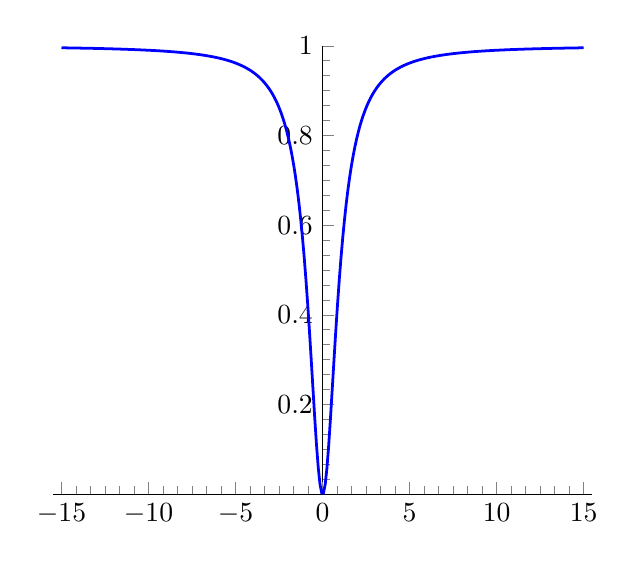
\begin{tikzpicture}
            \begin{axis}[
                ymin=0,
                ymax=1,
                xmin=-15.5, 
                xmax=15.5,
                minor tick num=5,
                axis lines*=middle,
                xtick align=inside,
                ytick align=inside,
                extra x ticks={0}
                ]       
                \addplot[blue, line width=1pt, domain=-15:15, samples=300] {x^2/(1+x^2)};
            \end{axis}
        \end{tikzpicture}
    \end{center}

    我们可以注意到,分母大于分子,因此,当 $x$ 越来越大时,这两个量相对来说会越来越接近(也就是说,它们的比率接近 $1$)。另外,由于这两项都涉及平方,所以它们都是非负的,其比率至少为 $0$。综上所述,我们可以得出以下结论:

    定义集合
    \[T = \{y \in \mathbb{R} \mid 0 \le y < 1\}\]
    我们声称 $T = Im_f (\mathbb{R})$。

    我们现在将沿用之前示例中采用的策略。在此之前,先回顾一下:证明的第二部分 --- 证明所声明的集合是像的子集 --- 是较为困难的部分。我们需要预见到这一点。

    在这部分中,我们将处理任意元素 $y \in T$,并希望找到一个元素 $x \in \mathbb{R}$,使得 $f(x) = y$。为了找到这样的 $x$,我们需要设定等式并尝试求解 $x$:
    \begin{align*}
        y = \frac{x^2}{1+x^2} &\iff  (1 + x^2)y = x^2 \\
        &\iff y + yx^2 - x^2 = 0 \\
        &\iff (y - 1)x^2 = -y \\
        &\iff x^2=\frac{y}{1-y} 
    \end{align*}
    那么现在怎么办?我们能确定 $\frac{y}{1-y} \in \mathbb{R}$ 吗?我们能确定它非负,从而确定存在这样的 $x$ 吗?关于可能存在两个根的问题呢?请思考这些潜在的问题,并在继续阅读我们的证明之前尝试写出你自己的版本!

    \begin{proof}
        首先,我们来证明 $Im_f (\mathbb{R}) \subseteq T$。

        设 $y \in Im_f (R)$ 为任意固定元素。根据像的定义,$\exists x \in \mathbb{R}$ 是的 $f(x) = y$。给定这样的 $x$。

        因为 $x \in \mathbb{R}$,我们知道 $x^2 \ge 0$ 且 $0 < x^2+1$,我们可以推导出 $0 < \frac{1}{x^2+1}$。

        由于所有项都是非负的,我们可以将之前的两个不等式相乘,从而推导出 $0 < \frac{x^2}{1+x^2}$。

        我们还知道 $0 \le x^2 < x^2 + 1$,所以 $\frac{x^2}{x^2+1}<1$。(备注,为什么指出 $x^2>0$ 很重要?不指出可能会出现什么问题?)

        这证明了 $0 \le \frac{x^2}{1+x^2} < 1$。因为 $y = f(x) = \frac{x^2}{1+x^2}$,这等价于 $0 \le y < 1$。

        因此 $y \in T$,所以 $Im_f (R) \subseteq T$。\\

        接着,我们来证明 $T \subseteq Im_f (\mathbb{R})$。

        设 $y \in T$ 为任意固定元素。这意味着 $y \in \mathbb{R}$ 且 $0 \le y < 1$。

        要证明 $y \in Im_f (\mathbb{R})$,我们需要得到一个 $x$ 满足 $f(x) = y$。

        我们声称 $x = \sqrt{\frac{y}{1-y}}$ 满足。

        请注意 $0 \le y < 1 \implies -y > -1$,所以 $1-y > 0$。因此 $\frac{y}{1-y} \ge 0$ 且 $x \in \mathbb{R}$ 可以明确定义为平方根,并且 $x$ 属于定义域 $\mathbb{R}$。
        
        注意到 $x^2=\frac{y}{1-y}$,所以
        \[f(x) = \frac{x^2}{1+x^2} = \frac{\frac{y}{1-y}}{1+\frac{y}{1-y}}\frac{\frac{y}{1-y}}{\frac{(1-y)+y}{1-y}}=\frac{\frac{y}{1-y}}{\frac{1}{1-y}}=\frac{y}{1-y} \cdot \frac{1-y}{1} = \frac{y}{1} = y\]
        这证明 $y \in Im_f (R)$,所以 $T \subseteq Im_f (R)$。\\

        综上,利用双重包含论证,我们得到结论 $T = Im_f (\mathbb{R})$。
    \end{proof}
\end{example}

请注意我们如何解决之前讨论的证明问题。是的,有两个潜在的 $x$ 值可以起作用(即正平方根和负平方根),但我们只需要一个,所以我们选择了正平方根并继续完成了证明。

(问题:如果这个函数只定义在非负实数上怎么办?如果只定义在负实数上呢?这种限制会如何影响我们的选择?)\\

\begin{example}
    考虑函数 $p:\mathbb{N} \times \mathbb{N} \to \mathbb{N}$ 定义为
    \[\forall (a, b) \in \mathbb{N} \times \mathbb{N} \centerdot p(a, b) = ab + a\]
    $Im_p(\mathbb{N})$ 是什么?

    这个例子可能会感觉有点棘手,因为它涉及到集合的笛卡尔积。也就是说,函数 $p$ 接受一对自然数作为输入,并输出一个自然数。在这种情况下,一个好的方法是先代入一些值,看看结果如何。请参考下面的数值表,左列表示 $a$ 的值,顶行表示 $b$ 的值,表格中的项是 $p(a, b)$ 的值。

    \begin{center}
        \begin{tabular}{c|ccccc}
              &  1 &  2 &  3 &  4 & 5  \\
            \hline
            1 &  2 &  3 &  4 &  5 & 6  \\
            2 &  4 &  6 &  8 & 10 & 12 \\
            3 &  6 &  9 & 12 & 15 & 18 \\
            4 &  8 & 12 & 16 & 20 & 24 \\
            5 & 10 & 15 & 20 & 25 & 30 \\
        \end{tabular}
    \end{center}

    看起来函数 $p$ ``得到了''除 $1$ 以外的所有自然数。具体来说,看一下数组第一行的值:除了 $1$ 以外,所有的自然数都在那里。我们可以在接下来的证明中运用这一洞察。

    \begin{proof}
        设 $V = N - \{1\}$。我们声称 $V = Im_p(\mathbb{N} \times \mathbb{N})$。

        首先,我们来证明 $Im_p(\mathbb{N} \times \mathbb{N}) \subseteq V$。

        设 $n \in Im_p(\mathbb{N} \times \mathbb{N})$ 为任意固定元素。这意味着 $n \in \mathbb{N}$ 且 $\exists (a,b) \in \mathbb{N} \times \mathbb{N}$ 使得 $p(a,b)=n$。给定这样的 $(a,b)$。

        这意味着 $n=ab+a$。因为 $a,b \ge 1$,所以 $ab \ge 1$ 所以 $n = ab + a \ge 2$。根据 $V$ 的定义,着证明了 $n \in V$。

        因此 $Im_p(\mathbb{N} \times \mathbb{N}) \subseteq V$。

        (在继续阅读我们的证明之前,试着自己写出证明的后半部分!)\\

        接着,我们来证明 $V \subseteq Im_p(\mathbb{N} \times \mathbb{N})$。

        设 $v \in V$ 为任意固定元素。这意味着 $v \in \mathbb{N}$ 且 $v \ge 2$。定义 $(a, b) = (v - 1, 1)$。

        注意,$v - 1 \ge 1$,所以 $v-1 \in \mathbb{N}$,因此 $(a, b) \in \mathbb{N} \times \mathbb{N}$。

        此外,我们还注意到
        \[p(a, b) = p(v - 1, 1) = (v - 1) \centerdot 1 + 1 = v - 1 + 1 = v\]
        
        因此 $p(a, b) = v$,所以 $(a,b) \in Im_p(\mathbb{N} \times \mathbb{N})$。
        
        因此 $V \subseteq Im_p(\mathbb{N} \times \mathbb{N})$。\\

        综上,利用双重包含论证,我们得到结论 $V = Im_p(\mathbb{N} \times \mathbb{N})$。
    \end{proof}
\end{example}